%=====================================================================
%  MMSS Graph Theory : Daily Report + Solutions
%
%  This is the only file you edit day to day.
%  All packages, styles and graph macros live in backend.tex.
%  Cheat sheet for the graph toolkit: top of backend.tex, or readme.txt.
%=====================================================================

\documentclass[11pt]{article}
%settings
\newcommand{\teamname}{[GROUP NAME]}
\newcommand{\reportdate}{\today}
\newcommand{\logopath}{assets/logo.png}  
\usepackage{float}


%=====================================================================
%  backend.tex : MMSS Graph Theory report engine
%
%  DO NOT edit this file for day-to-day reports. Edit main.tex.
%  Touch this file only when you want a NEW macro or a style change.
%  (Makers note : This was really hard to make and I strongly suggest 
%  you dont touch it T-T....)
%  Loaded by main.tex via %=====================================================================
%  backend.tex : MMSS Graph Theory report engine
%
%  DO NOT edit this file for day-to-day reports. Edit main.tex.
%  Touch this file only when you want a NEW macro or a style change.
%  (Makers note : This was really hard to make and I strongly suggest 
%  you dont touch it T-T....)
%  Loaded by main.tex via %=====================================================================
%  backend.tex : MMSS Graph Theory report engine
%
%  DO NOT edit this file for day-to-day reports. Edit main.tex.
%  Touch this file only when you want a NEW macro or a style change.
%  (Makers note : This was really hard to make and I strongly suggest 
%  you dont touch it T-T....)
%  Loaded by main.tex via \input{backend} (after \documentclass).
%
%  Expects (optionally) these to be defined in main.tex BEFORE \input:
%    \teamname    \reportdate    \logopath
%  Fallbacks are provided below, so nothing breaks if you forget.
%
%  ---------------------------------------------------------------
%  GRAPH TOOLKIT CHEAT SHEET  (all calls go INSIDE graphfig/tikzpicture)
%  ---------------------------------------------------------------
%    \gcycle{n}{radius}{prefix}      n vertices on a circle, joined as a cycle
%    \gcyclen{n}{radius}{prefix}     same, vertices labelled 1..n
%    \gcomplete{n}{radius}{prefix}   complete graph K_n on a circle
%    \gbipartite{m}{n}{gap}          complete bipartite K_{m,n}
%                                      handles: left bl1..blm, right br1..brn
%    \gpath{n}{spacing}{prefix}      path on n vertices, left to right
%    \gpetersen                      Petersen graph  (\gpeterson kept as alias)
%                                      handles: outer po0..po4, inner pin0..pin4
%    \gcube{n}                       n x n x n grid cube, oblique 2D projection
%    \gqgon{n}, \gpancake{n}         suprise hidden functions, only use after you 
%                                      learned what it is. 
%
%  Named handles stay live for the rest of the picture, so after a call:
%    \draw[edge,densely dashed] (po0)--(pin2);   or   \node[hv] at (bl1){};
%
%  Vertex styles:  v (filled dot) . ov (open ring) . hv (highlighted hub)
%  Edge style:     edge
%
%  Figure wrapper: \begin{graphfig}[scale]{Label} ... \end{graphfig}
%    {Text} -> centred, titled  [Graph Text]
%    {NUM}  -> centred, auto-numbered  [Graph 1], [Graph 2], ...
%    {}     -> bare, no title, no centring (use to line pictures up side by side)
%=====================================================================

\usepackage[margin=1in,headheight=30pt,headsep=16pt]{geometry}
\usepackage{amsmath,amssymb,amsfonts,amsthm}
\usepackage{enumitem}
\usepackage{fancyhdr}
\usepackage{hyperref}
\usepackage{graphicx}
\usepackage{tikz}
\usepackage{xcolor}
\usetikzlibrary{arrows.meta,calc}


\providecommand{\teamname}{[GROUP NAME]}
\providecommand{\reportdate}{\today}
\providecommand{\logopath}{assets/logo.png}

\pagestyle{fancy}
\fancyhf{}
\renewcommand{\headrulewidth}{0.4pt}
\renewcommand{\footrulewidth}{0pt}
\fancyhead[L]{\raisebox{2pt}{\small\textsc{\teamname}}}
\fancyhead[R]{\expandafter\IfFileExists\expandafter{\logopath}
  {\includegraphics[height=10pt]{\logopath}}{}}
\fancyfoot[C]{\small\thepage}

\fancypagestyle{firstpage}{
  \fancyhf{}
  \renewcommand{\headrulewidth}{0pt}
  \fancyfoot[C]{\small\thepage}
}

\setlength{\parindent}{0pt}
\setlength{\parskip}{6pt}

\newcommand{\divider}{\begin{center}\rule{0.6\textwidth}{0.4pt}\end{center}}

\newtheoremstyle{solstyle}{6pt}{6pt}{}{}{\bfseries}{.}{ }{}
\theoremstyle{solstyle}
\newtheorem*{solution}{Solution}

\newcommand{\WLoG}{WLoG}
\newcommand{\Cn}[1]{C_{#1}}
\newcommand{\Kn}[1]{K_{#1}}
\newcommand{\Kt}[2]{K_{#1,#2}}

\tikzset{
  v/.style ={circle, fill=black, inner sep=1.6pt},
  ov/.style={circle, draw=black, fill=white, line width=0.6pt, inner sep=1.6pt},
  hv/.style={circle, fill=black!55, draw=black, line width=0.6pt, inner sep=2.6pt},
  edge/.style={line width=0.6pt},
}


\newcommand{\gcycle}[3]{
  \foreach \gi in {1,...,#1}{\node[v] (#3\gi) at ({90-(\gi-1)*360/#1}:#2){};}
  \foreach \gi in {1,...,#1}{\pgfmathtruncatemacro{\gj}{mod(\gi,#1)+1}\draw[edge] (#3\gi)--(#3\gj);}
}

\newcommand{\gcyclen}[3]{
  \foreach \gi in {1,...,#1}{
    \pgfmathsetmacro{\gang}{90-(\gi-1)*360/#1}
    \node[v,label={\gang:\gi}] (#3\gi) at (\gang:#2){};}
  \foreach \gi in {1,...,#1}{\pgfmathtruncatemacro{\gj}{mod(\gi,#1)+1}\draw[edge] (#3\gi)--(#3\gj);}
}

\newcommand{\gcomplete}[3]{
  \foreach \gi in {1,...,#1}{\node[v] (#3\gi) at ({90-(\gi-1)*360/#1}:#2){};}
  \foreach \gi in {1,...,#1}{\foreach \gj in {1,...,#1}{\ifnum\gi<\gj\relax\draw[edge] (#3\gi)--(#3\gj);\fi}}
}

\newcommand{\gbipartite}[3]{
  \foreach \gi in {1,...,#1}{\node[v] (bl\gi) at (0,{(#1+1)/2-\gi}){};}
  \foreach \gj in {1,...,#2}{\node[v] (br\gj) at (#3,{(#2+1)/2-\gj}){};}
  \foreach \gi in {1,...,#1}{\foreach \gj in {1,...,#2}{\draw[edge] (bl\gi)--(br\gj);}}
}

\newcommand{\gpath}[3]{
  \foreach \gi in {1,...,#1}{\node[v] (#3\gi) at ({(\gi-1)*#2},0){};}
  \pgfmathtruncatemacro{\gplast}{#1-1}
  \foreach \gi in {1,...,\gplast}{\pgfmathtruncatemacro{\gpk}{\gi+1}\draw[edge] (#3\gi)--(#3\gpk);}
}


\newcommand{\gpetersen}{
  \foreach \gp in {0,...,4}{
    \node[v] (po\gp) at ({90+\gp*72}:2){};
    \node[v] (pin\gp) at ({90+\gp*72}:1){};}
  \foreach \gp in {0,...,4}{
    \pgfmathtruncatemacro{\gpj}{mod(\gp+1,5)}
    \pgfmathtruncatemacro{\gpk}{mod(\gp+2,5)}
    \draw[edge] (po\gp)--(po\gpj);
    \draw[edge] (po\gp)--(pin\gp);
    \draw[edge] (pin\gp)--(pin\gpk);
  }
}
\newcommand{\gpeterson}{\gpetersen}

\newcommand{\gcube}[1]{
  \begin{scope}[x={(1cm,0cm)}, y={(0cm,1cm)}, z={(0.5cm,0.45cm)}]
    \foreach \ci in {0,...,#1}{\draw[edge] (\ci,0,0)--(\ci,#1,0);}
    \foreach \cj in {0,...,#1}{\draw[edge] (0,\cj,0)--(#1,\cj,0);}
    \foreach \ci in {0,...,#1}{\draw[edge] (\ci,#1,0)--(\ci,#1,#1);}
    \foreach \ck in {0,...,#1}{\draw[edge] (0,#1,\ck)--(#1,#1,\ck);}
    \foreach \cj in {0,...,#1}{\draw[edge] (#1,\cj,0)--(#1,\cj,#1);}
    \foreach \ck in {0,...,#1}{\draw[edge] (#1,0,\ck)--(#1,#1,\ck);}
    \foreach \ci in {0,...,#1}{\foreach \cj in {0,...,#1}{\node[v] at (\ci,\cj,0){};}}
    \foreach \ci in {0,...,#1}{\foreach \ck in {0,...,#1}{\node[v] at (\ci,#1,\ck){};}}
    \foreach \cj in {0,...,#1}{\foreach \ck in {0,...,#1}{\node[v] at (#1,\cj,\ck){};}}
  \end{scope}
}

\newcount\pgPlaced
\newcount\pgNf
\newcount\pgTt
\newcommand{\gpancake}[2]{
  \pgNf=1 \pgTt=1
  \loop\ifnum\pgTt<#1 \advance\pgTt by1\relax \multiply\pgNf by\pgTt \repeat
  \edef\pgNfact{\the\pgNf}
  \pgfmathtruncatemacro{\pgTotm}{#1^#1-1}
  \pgPlaced=0
  \foreach \pgI in {0,...,\pgTotm}{
    \gdef\pgPerm{}\xdef\pgUsed{0}\xdef\pgValid{1}
    \foreach \pos in {1,...,#1}{
      \pgfmathtruncatemacro{\pgDig}{Mod(floor(\pgI/(#1^(#1-\pos))),#1)}
      \pgfmathtruncatemacro{\pgBit}{Mod(floor(\pgUsed/(2^\pgDig)),2)}
      \ifnum\pgBit=1 \xdef\pgValid{0}
      \else
        \pgfmathtruncatemacro{\pgNewUsed}{\pgUsed+2^\pgDig}\xdef\pgUsed{\pgNewUsed}
        \pgfmathtruncatemacro{\pgD}{\pgDig+1}\xdef\pgPerm{\pgPerm\pgD}
      \fi}
    \ifnum\pgValid=1
      \pgfmathsetmacro{\pgAng}{90-(\the\pgPlaced)*360/\pgNfact}
      \node[v,label={\pgAng:{\tiny\pgPerm}}] (p\pgPerm) at (\pgAng:#2){};
      \global\advance\pgPlaced by1\relax
    \fi}
  \foreach \pgI in {0,...,\pgTotm}{
    \gdef\pgPerm{}\xdef\pgUsed{0}\xdef\pgValid{1}
    \foreach \pos in {1,...,#1}{
      \pgfmathtruncatemacro{\pgDig}{Mod(floor(\pgI/(#1^(#1-\pos))),#1)}
      \pgfmathtruncatemacro{\pgBit}{Mod(floor(\pgUsed/(2^\pgDig)),2)}
      \ifnum\pgBit=1 \xdef\pgValid{0}
      \else
        \pgfmathtruncatemacro{\pgNewUsed}{\pgUsed+2^\pgDig}\xdef\pgUsed{\pgNewUsed}
        \pgfmathtruncatemacro{\pgD}{\pgDig+1}\xdef\pgPerm{\pgPerm\pgD}
        \expandafter\xdef\csname pgDig\pos\endcsname{\pgD}
      \fi}
    \ifnum\pgValid=1
      \foreach \k in {2,...,#1}{
        \xdef\pgNb{}
        \foreach \j in {1,...,\k}{\xdef\pgNb{\csname pgDig\j\endcsname\pgNb}}
        \ifnum\k<#1
          \foreach \j in {\the\numexpr\k+1\relax,...,#1}{\xdef\pgNb{\pgNb\csname pgDig\j\endcsname}}
        \fi
        \draw[edge] (p\pgPerm)--(p\pgNb);
      }
    \fi}
}




\newcommand{\gqgon}[2]{
  \pgfmathtruncatemacro{\Nm}{2^#1-1}
  \pgfmathtruncatemacro{\nm}{#1-1}
  \foreach \i in {0,...,\Nm}{
    \pgfmathsetmacro{\ang}{90-\i*360/(\Nm+1)}
    \xdef\lbl{}
    \foreach \k in {\nm,...,0}{
      \pgfmathtruncatemacro{\bit}{mod(floor(\i/(2^\k)),2)}
      \xdef\lbl{\lbl\bit}
    }
    \node[v,label={\ang:\scriptsize $\lbl$}] (q\i) at (\ang:#2){};
  }
  \foreach \i in {0,...,\Nm}{
    \foreach \k in {0,...,\nm}{
      \pgfmathtruncatemacro{\bit}{mod(floor(\i/(2^\k)),2)}
      \ifnum\bit=0
        \pgfmathtruncatemacro{\j}{\i+2^\k}
        \draw[edge] (q\i)--(q\j);
      \fi
    }
  }
}




\newcommand{\newinstructor}[2]{
  \definecolor{#2color}{HTML}{#1}
  \expandafter\newcommand\csname #2\endcsname[1]{
    {\color{#2color}\textbf{#2} : ##1}}}

\newcounter{graphnum}
\newif\ifgfbare
\def\gfEmpty{}
\def\gfNUM{NUM}
\newenvironment{graphfig}[2][1]{
  \def\gftmp{#2}
  \ifx\gftmp\gfEmpty
    \gfbaretrue
  \else
    \gfbarefalse
    \ifx\gftmp\gfNUM
      \stepcounter{graphnum}\edef\gflabel{\arabic{graphnum}}
    \else
      \def\gflabel{#2}
    \fi
  \fi
  \ifgfbare\else\begin{center}\fi
  \begin{tikzpicture}[scale=#1]
}{
  \end{tikzpicture}
  \ifgfbare\else\par\vspace{3pt}\textbf{[Graph \gflabel]}\end{center}\fi
}

\newcommand{\glabel}[1]{\begin{center}\textbf{[Graph #1]}\end{center}} (after \documentclass).
%
%  Expects (optionally) these to be defined in main.tex BEFORE \input:
%    \teamname    \reportdate    \logopath
%  Fallbacks are provided below, so nothing breaks if you forget.
%
%  ---------------------------------------------------------------
%  GRAPH TOOLKIT CHEAT SHEET  (all calls go INSIDE graphfig/tikzpicture)
%  ---------------------------------------------------------------
%    \gcycle{n}{radius}{prefix}      n vertices on a circle, joined as a cycle
%    \gcyclen{n}{radius}{prefix}     same, vertices labelled 1..n
%    \gcomplete{n}{radius}{prefix}   complete graph K_n on a circle
%    \gbipartite{m}{n}{gap}          complete bipartite K_{m,n}
%                                      handles: left bl1..blm, right br1..brn
%    \gpath{n}{spacing}{prefix}      path on n vertices, left to right
%    \gpetersen                      Petersen graph  (\gpeterson kept as alias)
%                                      handles: outer po0..po4, inner pin0..pin4
%    \gcube{n}                       n x n x n grid cube, oblique 2D projection
%    \gqgon{n}, \gpancake{n}         suprise hidden functions, only use after you 
%                                      learned what it is. 
%
%  Named handles stay live for the rest of the picture, so after a call:
%    \draw[edge,densely dashed] (po0)--(pin2);   or   \node[hv] at (bl1){};
%
%  Vertex styles:  v (filled dot) . ov (open ring) . hv (highlighted hub)
%  Edge style:     edge
%
%  Figure wrapper: \begin{graphfig}[scale]{Label} ... \end{graphfig}
%    {Text} -> centred, titled  [Graph Text]
%    {NUM}  -> centred, auto-numbered  [Graph 1], [Graph 2], ...
%    {}     -> bare, no title, no centring (use to line pictures up side by side)
%=====================================================================

\usepackage[margin=1in,headheight=30pt,headsep=16pt]{geometry}
\usepackage{amsmath,amssymb,amsfonts,amsthm}
\usepackage{enumitem}
\usepackage{fancyhdr}
\usepackage{hyperref}
\usepackage{graphicx}
\usepackage{tikz}
\usepackage{xcolor}
\usetikzlibrary{arrows.meta,calc}


\providecommand{\teamname}{[GROUP NAME]}
\providecommand{\reportdate}{\today}
\providecommand{\logopath}{assets/logo.png}

\pagestyle{fancy}
\fancyhf{}
\renewcommand{\headrulewidth}{0.4pt}
\renewcommand{\footrulewidth}{0pt}
\fancyhead[L]{\raisebox{2pt}{\small\textsc{\teamname}}}
\fancyhead[R]{\expandafter\IfFileExists\expandafter{\logopath}
  {\includegraphics[height=10pt]{\logopath}}{}}
\fancyfoot[C]{\small\thepage}

\fancypagestyle{firstpage}{
  \fancyhf{}
  \renewcommand{\headrulewidth}{0pt}
  \fancyfoot[C]{\small\thepage}
}

\setlength{\parindent}{0pt}
\setlength{\parskip}{6pt}

\newcommand{\divider}{\begin{center}\rule{0.6\textwidth}{0.4pt}\end{center}}

\newtheoremstyle{solstyle}{6pt}{6pt}{}{}{\bfseries}{.}{ }{}
\theoremstyle{solstyle}
\newtheorem*{solution}{Solution}

\newcommand{\WLoG}{WLoG}
\newcommand{\Cn}[1]{C_{#1}}
\newcommand{\Kn}[1]{K_{#1}}
\newcommand{\Kt}[2]{K_{#1,#2}}

\tikzset{
  v/.style ={circle, fill=black, inner sep=1.6pt},
  ov/.style={circle, draw=black, fill=white, line width=0.6pt, inner sep=1.6pt},
  hv/.style={circle, fill=black!55, draw=black, line width=0.6pt, inner sep=2.6pt},
  edge/.style={line width=0.6pt},
}


\newcommand{\gcycle}[3]{
  \foreach \gi in {1,...,#1}{\node[v] (#3\gi) at ({90-(\gi-1)*360/#1}:#2){};}
  \foreach \gi in {1,...,#1}{\pgfmathtruncatemacro{\gj}{mod(\gi,#1)+1}\draw[edge] (#3\gi)--(#3\gj);}
}

\newcommand{\gcyclen}[3]{
  \foreach \gi in {1,...,#1}{
    \pgfmathsetmacro{\gang}{90-(\gi-1)*360/#1}
    \node[v,label={\gang:\gi}] (#3\gi) at (\gang:#2){};}
  \foreach \gi in {1,...,#1}{\pgfmathtruncatemacro{\gj}{mod(\gi,#1)+1}\draw[edge] (#3\gi)--(#3\gj);}
}

\newcommand{\gcomplete}[3]{
  \foreach \gi in {1,...,#1}{\node[v] (#3\gi) at ({90-(\gi-1)*360/#1}:#2){};}
  \foreach \gi in {1,...,#1}{\foreach \gj in {1,...,#1}{\ifnum\gi<\gj\relax\draw[edge] (#3\gi)--(#3\gj);\fi}}
}

\newcommand{\gbipartite}[3]{
  \foreach \gi in {1,...,#1}{\node[v] (bl\gi) at (0,{(#1+1)/2-\gi}){};}
  \foreach \gj in {1,...,#2}{\node[v] (br\gj) at (#3,{(#2+1)/2-\gj}){};}
  \foreach \gi in {1,...,#1}{\foreach \gj in {1,...,#2}{\draw[edge] (bl\gi)--(br\gj);}}
}

\newcommand{\gpath}[3]{
  \foreach \gi in {1,...,#1}{\node[v] (#3\gi) at ({(\gi-1)*#2},0){};}
  \pgfmathtruncatemacro{\gplast}{#1-1}
  \foreach \gi in {1,...,\gplast}{\pgfmathtruncatemacro{\gpk}{\gi+1}\draw[edge] (#3\gi)--(#3\gpk);}
}


\newcommand{\gpetersen}{
  \foreach \gp in {0,...,4}{
    \node[v] (po\gp) at ({90+\gp*72}:2){};
    \node[v] (pin\gp) at ({90+\gp*72}:1){};}
  \foreach \gp in {0,...,4}{
    \pgfmathtruncatemacro{\gpj}{mod(\gp+1,5)}
    \pgfmathtruncatemacro{\gpk}{mod(\gp+2,5)}
    \draw[edge] (po\gp)--(po\gpj);
    \draw[edge] (po\gp)--(pin\gp);
    \draw[edge] (pin\gp)--(pin\gpk);
  }
}
\newcommand{\gpeterson}{\gpetersen}

\newcommand{\gcube}[1]{
  \begin{scope}[x={(1cm,0cm)}, y={(0cm,1cm)}, z={(0.5cm,0.45cm)}]
    \foreach \ci in {0,...,#1}{\draw[edge] (\ci,0,0)--(\ci,#1,0);}
    \foreach \cj in {0,...,#1}{\draw[edge] (0,\cj,0)--(#1,\cj,0);}
    \foreach \ci in {0,...,#1}{\draw[edge] (\ci,#1,0)--(\ci,#1,#1);}
    \foreach \ck in {0,...,#1}{\draw[edge] (0,#1,\ck)--(#1,#1,\ck);}
    \foreach \cj in {0,...,#1}{\draw[edge] (#1,\cj,0)--(#1,\cj,#1);}
    \foreach \ck in {0,...,#1}{\draw[edge] (#1,0,\ck)--(#1,#1,\ck);}
    \foreach \ci in {0,...,#1}{\foreach \cj in {0,...,#1}{\node[v] at (\ci,\cj,0){};}}
    \foreach \ci in {0,...,#1}{\foreach \ck in {0,...,#1}{\node[v] at (\ci,#1,\ck){};}}
    \foreach \cj in {0,...,#1}{\foreach \ck in {0,...,#1}{\node[v] at (#1,\cj,\ck){};}}
  \end{scope}
}

\newcount\pgPlaced
\newcount\pgNf
\newcount\pgTt
\newcommand{\gpancake}[2]{
  \pgNf=1 \pgTt=1
  \loop\ifnum\pgTt<#1 \advance\pgTt by1\relax \multiply\pgNf by\pgTt \repeat
  \edef\pgNfact{\the\pgNf}
  \pgfmathtruncatemacro{\pgTotm}{#1^#1-1}
  \pgPlaced=0
  \foreach \pgI in {0,...,\pgTotm}{
    \gdef\pgPerm{}\xdef\pgUsed{0}\xdef\pgValid{1}
    \foreach \pos in {1,...,#1}{
      \pgfmathtruncatemacro{\pgDig}{Mod(floor(\pgI/(#1^(#1-\pos))),#1)}
      \pgfmathtruncatemacro{\pgBit}{Mod(floor(\pgUsed/(2^\pgDig)),2)}
      \ifnum\pgBit=1 \xdef\pgValid{0}
      \else
        \pgfmathtruncatemacro{\pgNewUsed}{\pgUsed+2^\pgDig}\xdef\pgUsed{\pgNewUsed}
        \pgfmathtruncatemacro{\pgD}{\pgDig+1}\xdef\pgPerm{\pgPerm\pgD}
      \fi}
    \ifnum\pgValid=1
      \pgfmathsetmacro{\pgAng}{90-(\the\pgPlaced)*360/\pgNfact}
      \node[v,label={\pgAng:{\tiny\pgPerm}}] (p\pgPerm) at (\pgAng:#2){};
      \global\advance\pgPlaced by1\relax
    \fi}
  \foreach \pgI in {0,...,\pgTotm}{
    \gdef\pgPerm{}\xdef\pgUsed{0}\xdef\pgValid{1}
    \foreach \pos in {1,...,#1}{
      \pgfmathtruncatemacro{\pgDig}{Mod(floor(\pgI/(#1^(#1-\pos))),#1)}
      \pgfmathtruncatemacro{\pgBit}{Mod(floor(\pgUsed/(2^\pgDig)),2)}
      \ifnum\pgBit=1 \xdef\pgValid{0}
      \else
        \pgfmathtruncatemacro{\pgNewUsed}{\pgUsed+2^\pgDig}\xdef\pgUsed{\pgNewUsed}
        \pgfmathtruncatemacro{\pgD}{\pgDig+1}\xdef\pgPerm{\pgPerm\pgD}
        \expandafter\xdef\csname pgDig\pos\endcsname{\pgD}
      \fi}
    \ifnum\pgValid=1
      \foreach \k in {2,...,#1}{
        \xdef\pgNb{}
        \foreach \j in {1,...,\k}{\xdef\pgNb{\csname pgDig\j\endcsname\pgNb}}
        \ifnum\k<#1
          \foreach \j in {\the\numexpr\k+1\relax,...,#1}{\xdef\pgNb{\pgNb\csname pgDig\j\endcsname}}
        \fi
        \draw[edge] (p\pgPerm)--(p\pgNb);
      }
    \fi}
}




\newcommand{\gqgon}[2]{
  \pgfmathtruncatemacro{\Nm}{2^#1-1}
  \pgfmathtruncatemacro{\nm}{#1-1}
  \foreach \i in {0,...,\Nm}{
    \pgfmathsetmacro{\ang}{90-\i*360/(\Nm+1)}
    \xdef\lbl{}
    \foreach \k in {\nm,...,0}{
      \pgfmathtruncatemacro{\bit}{mod(floor(\i/(2^\k)),2)}
      \xdef\lbl{\lbl\bit}
    }
    \node[v,label={\ang:\scriptsize $\lbl$}] (q\i) at (\ang:#2){};
  }
  \foreach \i in {0,...,\Nm}{
    \foreach \k in {0,...,\nm}{
      \pgfmathtruncatemacro{\bit}{mod(floor(\i/(2^\k)),2)}
      \ifnum\bit=0
        \pgfmathtruncatemacro{\j}{\i+2^\k}
        \draw[edge] (q\i)--(q\j);
      \fi
    }
  }
}




\newcommand{\newinstructor}[2]{
  \definecolor{#2color}{HTML}{#1}
  \expandafter\newcommand\csname #2\endcsname[1]{
    {\color{#2color}\textbf{#2} : ##1}}}

\newcounter{graphnum}
\newif\ifgfbare
\def\gfEmpty{}
\def\gfNUM{NUM}
\newenvironment{graphfig}[2][1]{
  \def\gftmp{#2}
  \ifx\gftmp\gfEmpty
    \gfbaretrue
  \else
    \gfbarefalse
    \ifx\gftmp\gfNUM
      \stepcounter{graphnum}\edef\gflabel{\arabic{graphnum}}
    \else
      \def\gflabel{#2}
    \fi
  \fi
  \ifgfbare\else\begin{center}\fi
  \begin{tikzpicture}[scale=#1]
}{
  \end{tikzpicture}
  \ifgfbare\else\par\vspace{3pt}\textbf{[Graph \gflabel]}\end{center}\fi
}

\newcommand{\glabel}[1]{\begin{center}\textbf{[Graph #1]}\end{center}} (after \documentclass).
%
%  Expects (optionally) these to be defined in main.tex BEFORE \input:
%    \teamname    \reportdate    \logopath
%  Fallbacks are provided below, so nothing breaks if you forget.
%
%  ---------------------------------------------------------------
%  GRAPH TOOLKIT CHEAT SHEET  (all calls go INSIDE graphfig/tikzpicture)
%  ---------------------------------------------------------------
%    \gcycle{n}{radius}{prefix}      n vertices on a circle, joined as a cycle
%    \gcyclen{n}{radius}{prefix}     same, vertices labelled 1..n
%    \gcomplete{n}{radius}{prefix}   complete graph K_n on a circle
%    \gbipartite{m}{n}{gap}          complete bipartite K_{m,n}
%                                      handles: left bl1..blm, right br1..brn
%    \gpath{n}{spacing}{prefix}      path on n vertices, left to right
%    \gpetersen                      Petersen graph  (\gpeterson kept as alias)
%                                      handles: outer po0..po4, inner pin0..pin4
%    \gcube{n}                       n x n x n grid cube, oblique 2D projection
%    \gqgon{n}, \gpancake{n}         suprise hidden functions, only use after you 
%                                      learned what it is. 
%
%  Named handles stay live for the rest of the picture, so after a call:
%    \draw[edge,densely dashed] (po0)--(pin2);   or   \node[hv] at (bl1){};
%
%  Vertex styles:  v (filled dot) . ov (open ring) . hv (highlighted hub)
%  Edge style:     edge
%
%  Figure wrapper: \begin{graphfig}[scale]{Label} ... \end{graphfig}
%    {Text} -> centred, titled  [Graph Text]
%    {NUM}  -> centred, auto-numbered  [Graph 1], [Graph 2], ...
%    {}     -> bare, no title, no centring (use to line pictures up side by side)
%=====================================================================

\usepackage[margin=1in,headheight=30pt,headsep=16pt]{geometry}
\usepackage{amsmath,amssymb,amsfonts,amsthm}
\usepackage{enumitem}
\usepackage{fancyhdr}
\usepackage{hyperref}
\usepackage{graphicx}
\usepackage{tikz}
\usepackage{xcolor}
\usetikzlibrary{arrows.meta,calc}


\providecommand{\teamname}{[GROUP NAME]}
\providecommand{\reportdate}{\today}
\providecommand{\logopath}{assets/logo.png}

\pagestyle{fancy}
\fancyhf{}
\renewcommand{\headrulewidth}{0.4pt}
\renewcommand{\footrulewidth}{0pt}
\fancyhead[L]{\raisebox{2pt}{\small\textsc{\teamname}}}
\fancyhead[R]{\expandafter\IfFileExists\expandafter{\logopath}
  {\includegraphics[height=10pt]{\logopath}}{}}
\fancyfoot[C]{\small\thepage}

\fancypagestyle{firstpage}{
  \fancyhf{}
  \renewcommand{\headrulewidth}{0pt}
  \fancyfoot[C]{\small\thepage}
}

\setlength{\parindent}{0pt}
\setlength{\parskip}{6pt}

\newcommand{\divider}{\begin{center}\rule{0.6\textwidth}{0.4pt}\end{center}}

\newtheoremstyle{solstyle}{6pt}{6pt}{}{}{\bfseries}{.}{ }{}
\theoremstyle{solstyle}
\newtheorem*{solution}{Solution}

\newcommand{\WLoG}{WLoG}
\newcommand{\Cn}[1]{C_{#1}}
\newcommand{\Kn}[1]{K_{#1}}
\newcommand{\Kt}[2]{K_{#1,#2}}

\tikzset{
  v/.style ={circle, fill=black, inner sep=1.6pt},
  ov/.style={circle, draw=black, fill=white, line width=0.6pt, inner sep=1.6pt},
  hv/.style={circle, fill=black!55, draw=black, line width=0.6pt, inner sep=2.6pt},
  edge/.style={line width=0.6pt},
}


\newcommand{\gcycle}[3]{
  \foreach \gi in {1,...,#1}{\node[v] (#3\gi) at ({90-(\gi-1)*360/#1}:#2){};}
  \foreach \gi in {1,...,#1}{\pgfmathtruncatemacro{\gj}{mod(\gi,#1)+1}\draw[edge] (#3\gi)--(#3\gj);}
}

\newcommand{\gcyclen}[3]{
  \foreach \gi in {1,...,#1}{
    \pgfmathsetmacro{\gang}{90-(\gi-1)*360/#1}
    \node[v,label={\gang:\gi}] (#3\gi) at (\gang:#2){};}
  \foreach \gi in {1,...,#1}{\pgfmathtruncatemacro{\gj}{mod(\gi,#1)+1}\draw[edge] (#3\gi)--(#3\gj);}
}

\newcommand{\gcomplete}[3]{
  \foreach \gi in {1,...,#1}{\node[v] (#3\gi) at ({90-(\gi-1)*360/#1}:#2){};}
  \foreach \gi in {1,...,#1}{\foreach \gj in {1,...,#1}{\ifnum\gi<\gj\relax\draw[edge] (#3\gi)--(#3\gj);\fi}}
}

\newcommand{\gbipartite}[3]{
  \foreach \gi in {1,...,#1}{\node[v] (bl\gi) at (0,{(#1+1)/2-\gi}){};}
  \foreach \gj in {1,...,#2}{\node[v] (br\gj) at (#3,{(#2+1)/2-\gj}){};}
  \foreach \gi in {1,...,#1}{\foreach \gj in {1,...,#2}{\draw[edge] (bl\gi)--(br\gj);}}
}

\newcommand{\gpath}[3]{
  \foreach \gi in {1,...,#1}{\node[v] (#3\gi) at ({(\gi-1)*#2},0){};}
  \pgfmathtruncatemacro{\gplast}{#1-1}
  \foreach \gi in {1,...,\gplast}{\pgfmathtruncatemacro{\gpk}{\gi+1}\draw[edge] (#3\gi)--(#3\gpk);}
}


\newcommand{\gpetersen}{
  \foreach \gp in {0,...,4}{
    \node[v] (po\gp) at ({90+\gp*72}:2){};
    \node[v] (pin\gp) at ({90+\gp*72}:1){};}
  \foreach \gp in {0,...,4}{
    \pgfmathtruncatemacro{\gpj}{mod(\gp+1,5)}
    \pgfmathtruncatemacro{\gpk}{mod(\gp+2,5)}
    \draw[edge] (po\gp)--(po\gpj);
    \draw[edge] (po\gp)--(pin\gp);
    \draw[edge] (pin\gp)--(pin\gpk);
  }
}
\newcommand{\gpeterson}{\gpetersen}

\newcommand{\gcube}[1]{
  \begin{scope}[x={(1cm,0cm)}, y={(0cm,1cm)}, z={(0.5cm,0.45cm)}]
    \foreach \ci in {0,...,#1}{\draw[edge] (\ci,0,0)--(\ci,#1,0);}
    \foreach \cj in {0,...,#1}{\draw[edge] (0,\cj,0)--(#1,\cj,0);}
    \foreach \ci in {0,...,#1}{\draw[edge] (\ci,#1,0)--(\ci,#1,#1);}
    \foreach \ck in {0,...,#1}{\draw[edge] (0,#1,\ck)--(#1,#1,\ck);}
    \foreach \cj in {0,...,#1}{\draw[edge] (#1,\cj,0)--(#1,\cj,#1);}
    \foreach \ck in {0,...,#1}{\draw[edge] (#1,0,\ck)--(#1,#1,\ck);}
    \foreach \ci in {0,...,#1}{\foreach \cj in {0,...,#1}{\node[v] at (\ci,\cj,0){};}}
    \foreach \ci in {0,...,#1}{\foreach \ck in {0,...,#1}{\node[v] at (\ci,#1,\ck){};}}
    \foreach \cj in {0,...,#1}{\foreach \ck in {0,...,#1}{\node[v] at (#1,\cj,\ck){};}}
  \end{scope}
}

\newcount\pgPlaced
\newcount\pgNf
\newcount\pgTt
\newcommand{\gpancake}[2]{
  \pgNf=1 \pgTt=1
  \loop\ifnum\pgTt<#1 \advance\pgTt by1\relax \multiply\pgNf by\pgTt \repeat
  \edef\pgNfact{\the\pgNf}
  \pgfmathtruncatemacro{\pgTotm}{#1^#1-1}
  \pgPlaced=0
  \foreach \pgI in {0,...,\pgTotm}{
    \gdef\pgPerm{}\xdef\pgUsed{0}\xdef\pgValid{1}
    \foreach \pos in {1,...,#1}{
      \pgfmathtruncatemacro{\pgDig}{Mod(floor(\pgI/(#1^(#1-\pos))),#1)}
      \pgfmathtruncatemacro{\pgBit}{Mod(floor(\pgUsed/(2^\pgDig)),2)}
      \ifnum\pgBit=1 \xdef\pgValid{0}
      \else
        \pgfmathtruncatemacro{\pgNewUsed}{\pgUsed+2^\pgDig}\xdef\pgUsed{\pgNewUsed}
        \pgfmathtruncatemacro{\pgD}{\pgDig+1}\xdef\pgPerm{\pgPerm\pgD}
      \fi}
    \ifnum\pgValid=1
      \pgfmathsetmacro{\pgAng}{90-(\the\pgPlaced)*360/\pgNfact}
      \node[v,label={\pgAng:{\tiny\pgPerm}}] (p\pgPerm) at (\pgAng:#2){};
      \global\advance\pgPlaced by1\relax
    \fi}
  \foreach \pgI in {0,...,\pgTotm}{
    \gdef\pgPerm{}\xdef\pgUsed{0}\xdef\pgValid{1}
    \foreach \pos in {1,...,#1}{
      \pgfmathtruncatemacro{\pgDig}{Mod(floor(\pgI/(#1^(#1-\pos))),#1)}
      \pgfmathtruncatemacro{\pgBit}{Mod(floor(\pgUsed/(2^\pgDig)),2)}
      \ifnum\pgBit=1 \xdef\pgValid{0}
      \else
        \pgfmathtruncatemacro{\pgNewUsed}{\pgUsed+2^\pgDig}\xdef\pgUsed{\pgNewUsed}
        \pgfmathtruncatemacro{\pgD}{\pgDig+1}\xdef\pgPerm{\pgPerm\pgD}
        \expandafter\xdef\csname pgDig\pos\endcsname{\pgD}
      \fi}
    \ifnum\pgValid=1
      \foreach \k in {2,...,#1}{
        \xdef\pgNb{}
        \foreach \j in {1,...,\k}{\xdef\pgNb{\csname pgDig\j\endcsname\pgNb}}
        \ifnum\k<#1
          \foreach \j in {\the\numexpr\k+1\relax,...,#1}{\xdef\pgNb{\pgNb\csname pgDig\j\endcsname}}
        \fi
        \draw[edge] (p\pgPerm)--(p\pgNb);
      }
    \fi}
}




\newcommand{\gqgon}[2]{
  \pgfmathtruncatemacro{\Nm}{2^#1-1}
  \pgfmathtruncatemacro{\nm}{#1-1}
  \foreach \i in {0,...,\Nm}{
    \pgfmathsetmacro{\ang}{90-\i*360/(\Nm+1)}
    \xdef\lbl{}
    \foreach \k in {\nm,...,0}{
      \pgfmathtruncatemacro{\bit}{mod(floor(\i/(2^\k)),2)}
      \xdef\lbl{\lbl\bit}
    }
    \node[v,label={\ang:\scriptsize $\lbl$}] (q\i) at (\ang:#2){};
  }
  \foreach \i in {0,...,\Nm}{
    \foreach \k in {0,...,\nm}{
      \pgfmathtruncatemacro{\bit}{mod(floor(\i/(2^\k)),2)}
      \ifnum\bit=0
        \pgfmathtruncatemacro{\j}{\i+2^\k}
        \draw[edge] (q\i)--(q\j);
      \fi
    }
  }
}




\newcommand{\newinstructor}[2]{
  \definecolor{#2color}{HTML}{#1}
  \expandafter\newcommand\csname #2\endcsname[1]{
    {\color{#2color}\textbf{#2} : ##1}}}

\newcounter{graphnum}
\newif\ifgfbare
\def\gfEmpty{}
\def\gfNUM{NUM}
\newenvironment{graphfig}[2][1]{
  \def\gftmp{#2}
  \ifx\gftmp\gfEmpty
    \gfbaretrue
  \else
    \gfbarefalse
    \ifx\gftmp\gfNUM
      \stepcounter{graphnum}\edef\gflabel{\arabic{graphnum}}
    \else
      \def\gflabel{#2}
    \fi
  \fi
  \ifgfbare\else\begin{center}\fi
  \begin{tikzpicture}[scale=#1]
}{
  \end{tikzpicture}
  \ifgfbare\else\par\vspace{3pt}\textbf{[Graph \gflabel]}\end{center}\fi
}

\newcommand{\glabel}[1]{\begin{center}\textbf{[Graph #1]}\end{center}}

\begin{document}
\thispagestyle{firstpage}

%frontmatter
\noindent\textbf{\teamname}\hfill\textbf{\reportdate}

\noindent\textbf{Clarifier:} Changhwan\\
\textbf{Manager:} Benjamin\\
\textbf{Reporter:} Sharan\\
\textbf{Skeptic:} Henry

\textbf{Report:} Today we worked well as a team, covering a lot of problems quickly, which was an improvement over last time. It allowed us to spend more time on the harder questions.

% Instructor comments, if any:
%   \newinstructor{FF6600}{john}   in the settings area or right here
%   then use   \john{lorem ipsum}
%=====================================================================

\divider

\color{blue}Rachel is blue. \color{black}

\textbf{SOLUTIONS \& PROOFS:}\\
% Any extra notes to the reader go here.
Without Loss of Generality is abbreviated as \WLoG{} within this document.

%problems
\begin{enumerate}[leftmargin=*]

\item Find the five invariants for the following graph. 
\begin{graphfig}{NUM}[scale=0.8]
    \node [v] (a1) at (0,0){};
    \node [v] (a2) at (-4, 2){};
    \node [v] (a3) at (-2, 2){};
    \node [v] (a4) at (0, 2){};
    \node [v] (a5) at (2, 2){};
    \node [v] (a6) at (4, 2){};
    \node [v] (a7) at (-4, 4){};
    \node [v] (a8) at (-2, 4){};
    \node [v] (a9) at (0, 4){};
    \node [v] (a10) at (2, 4){};
    \node [v] (a11) at (4, 4){}; 
    \node [v] (a12) at (-3, 5){};
    \node [v] (a13) at (3, 5){};
    \draw (a1)--(a2)--(a3)--(a4)--(a5)--(a6)--(a11)--(a10)--(a9)--(a8)--(a7)--(a2);
    \draw (a3)--(a8) (a5)--(a10) (a3)--(a9) (a4)--(a10) (a6)--(a1) (a7)--(a12)--(a8) (a10)--(a13)--(a11) (a12)--(a9);
    \draw (a2)--(a8)--(a7)--(a3)--(a12)--(a2);
    \draw (a5)--(a11)--(a10)--(a6)--(a13)--(a5);
\end{graphfig}
\begin{solution}
$\chi(G)=5 , \alpha(G)=5, \omega(G)=5, \theta(G)=5, dom=2$
\end{solution}
\begin{proof}
\begin{enumerate}
    \item $\chi(G)$
        \begin{graphfig}{NUM}
            \node [v, fill=blue!100]    (a1)  at (0,0)  {};
            \node [v, fill=red!100]     (a2)  at (-4,2) {};
            \node [v, fill=purple!100]  (a3)  at (-2,2) {};
            \node [v, fill=blue!100]    (a4)  at (0,2)  {};
            \node [v, fill=red!100]     (a5)  at (2,2)  {};
            \node [v, fill=orange!100]   (a6)  at (4,2)  {};
            \node [v, fill=orange!100]   (a7)  at (-4,4) {};
            \node [v, fill=magenta!100] (a8)  at (-2,4) {};
            \node [v, fill=red!100]     (a9)  at (0,4)  {};
            \node [v, fill=purple!100]  (a10) at (2,4)  {};
            \node [v, fill=blue!100]    (a11) at (4,4)  {};
            \node [v, fill=blue!100]    (a12) at (-3,5) {};
            \node [v, fill=magenta!100] (a13) at (3,5)  {};
            \draw (a1)--(a2)--(a3)--(a4)--(a5)--(a6)--(a11)--(a10)--(a9)--(a8)--(a7)--(a2);
            \draw (a3)--(a8) (a5)--(a10) (a3)--(a9) (a4)--(a10) (a6)--(a1) (a7)--(a12)--(a8) (a10)--(a13)--(a11) (a12)--(a9);
            \draw (a2)--(a8)--(a7)--(a3)--(a12)--(a2);
            \draw (a5)--(a11)--(a10)--(a6)--(a13)--(a5);
        \end{graphfig}
        Therefore 5. Since there is a $K_5$, we know the minima of $\chi(G)$ is 5, and since we have shown a solution, it is valid. \color{red}The three kinda reds are hard to tell apart but this works!\color{black}
        \item $\alpha(G)$
        \begin{graphfig}{NUM}
            \node [hv] (a1) at (0,0){};
            \node [v] (a2) at (-4, 2){};
            \node [v] (a3) at (-2, 2){};
            \node [hv] (a4) at (0, 2){};
            \node [v] (a5) at (2, 2){};
            \node [v] (a6) at (4, 2){};
            \node [hv] (a7) at (-4, 4){};
            \node [v] (a8) at (-2, 4){};
            \node [hv] (a9) at (0, 4){};
            \node [v] (a10) at (2, 4){};
            \node [hv] (a11) at (4, 4){}; 
            \node [v] (a12) at (-3, 5){};
            \node [v] (a13) at (3, 5){};
            \draw (a1)--(a2)--(a3)--(a4)--(a5)--(a6)--(a11)--(a10)--(a9)--(a8)--(a7)--(a2);
            \draw (a3)--(a8) (a5)--(a10) (a3)--(a9) (a4)--(a10) (a6)--(a1) (a7)--(a12)--(a8) (a10)--(a13)--(a11) (a12)--(a9);
            \draw (a2)--(a8)--(a7)--(a3)--(a12)--(a2);
            \draw (a5)--(a11)--(a10)--(a6)--(a13)--(a5);
        \end{graphfig}
        Therefore 5. \color{red}Yeah, this is maximal due to clique partition number.\color{black}
        \item $\omega(G)$
        \begin{graphfig}{NUM}
            \node [v] (a1) at (0,0){};
            \node [hv] (a2) at (-4, 2){};
            \node [hv] (a3) at (-2, 2){};
            \node [v] (a4) at (0, 2){};
            \node [v] (a5) at (2, 2){};
            \node [v] (a6) at (4, 2){};
            \node [hv] (a7) at (-4, 4){};
            \node [hv] (a8) at (-2, 4){};
            \node [v] (a9) at (0, 4){};
            \node [v] (a10) at (2, 4){};
            \node [v] (a11) at (4, 4){}; 
            \node [hv] (a12) at (-3, 5){};
            \node [v] (a13) at (3, 5){};
            \draw (a1)--(a2)--(a3)--(a4)--(a5)--(a6)--(a11)--(a10)--(a9)--(a8)--(a7)--(a2);
            \draw (a3)--(a8) (a5)--(a10) (a3)--(a9) (a4)--(a10) (a6)--(a1) (a7)--(a12)--(a8) (a10)--(a13)--(a11) (a12)--(a9);
            \draw (a2)--(a8)--(a7)--(a3)--(a12)--(a2);
            \draw (a5)--(a11)--(a10)--(a6)--(a13)--(a5);
        \end{graphfig}
        Therefore 5. \color{red}\color{black}
        \item $\theta(G)$
        \begin{graphfig}{NUM}
            \node [v, fill=red!100]    (a1)  at (0,0)  {};
            \node [v, fill=blue!100]     (a2)  at (-4,2) {};
            \node [v, fill=purple!100]  (a3)  at (-2,2) {};
            \node [v, fill=orange!100]    (a4)  at (0,2)  {};
            \node [v, fill=orange!100]     (a5)  at (2,2)  {};
            \node [v, fill=magenta!100]   (a6)  at (4,2)  {};
            \node [v, fill=blue!100]   (a7)  at (-4,4) {};
            \node [v, fill=purple!100] (a8)  at (-2,4) {};
            \node [v, fill=purple!100]     (a9)  at (0,4)  {};
            \node [v, fill=orange!100]  (a10) at (2,4)  {};
            \node [v, fill=magenta!100]    (a11) at (4,4)  {};
            \node [v, fill=blue!100]    (a12) at (-3,5) {};
            \node [v, fill=magenta!100] (a13) at (3,5)  {};
            \draw (a1)--(a2)--(a3)--(a4)--(a5)--(a6)--(a11)--(a10)--(a9)--(a8)--(a7)--(a2);
            \draw (a3)--(a8) (a5)--(a10) (a3)--(a9) (a4)--(a10) (a6)--(a1) (a7)--(a12)--(a8) (a10)--(a13)--(a11) (a12)--(a9);
            \draw (a2)--(a8)--(a7)--(a3)--(a12)--(a2);
            \draw (a5)--(a11)--(a10)--(a6)--(a13)--(a5);
            \draw [blue] (a2)--(a7)--(a12)--(a2);
            \draw [purple] (a3)--(a8)--(a9)--(a3);
            \draw [orange] (a4)--(a10)--(a5)--(a4);
            \draw [magenta] (a6)--(a11)--(a13)--(a6);
        \end{graphfig}
        Therefore 5. 
        \item $\text{dom}(G)$
        \begin{graphfig}{NUM}
            \node [v, fill=red!100] (a1) at (0,0){};
            \node [hv, fill=red!100] (a2) at (-4, 2){};
            \node [v, fill=red!100] (a3) at (-2, 2){};
            \node [v, fill=blue!100] (a4) at (0, 2){};
            \node [v, fill=blue!100] (a5) at (2, 2){};
            \node [v, fill=blue!100] (a6) at (4, 2){};
            \node [v, fill=red!100] (a7) at (-4, 4){};
            \node [v, fill=red!100] (a8) at (-2, 4){};
            \node [v, fill=blue!100] (a9) at (0, 4){};
            \node [hv, fill=blue!100] (a10) at (2, 4){};
            \node [v, fill=blue!100] (a11) at (4, 4){}; 
            \node [v, fill=red!100] (a12) at (-3, 5){};
            \node [v, fill=blue!100] (a13) at (3, 5){};
            \draw (a1)--(a2)--(a3)--(a4)--(a5)--(a6)--(a11)--(a10)--(a9)--(a8)--(a7)--(a2);
            \draw (a3)--(a8) (a5)--(a10) (a3)--(a9) (a4)--(a10) (a6)--(a1) (a7)--(a12)--(a8) (a10)--(a13)--(a11) (a12)--(a9);
            \draw (a2)--(a8)--(a7)--(a3)--(a12)--(a2);
            \draw (a5)--(a11)--(a10)--(a6)--(a13)--(a5);
        \end{graphfig}
        Therefore 2. \color{red}Good! Finding the ends of the graphs was hard in the TeX though.\color{black}
\end{enumerate}
\end{proof}
\item Professor Shaw is hosting a party! Unfortunately, a lot of his friends and family hate each other. Professor Shaw has to make a graph where each friend/family member gets a vertex, and an edge goes between any two that hate each other. 
\begin{enumerate}[label=\alph*.]
    \item Assume that I want to have as many people as possible at my party, but that if I invite someone, I will not invite anyone (s)he hates. Which of the following quantities is most relevant? Why? 
    \begin{enumerate}
        \item $\chi(G)$
        \item \color{red}Solution. $\alpha(G)$\color{black}
        \item $\omega(G)$
        \item $\theta(G)$
        \item $\text{dom}(G)$
    \end{enumerate}
    \begin{proof}
        We don't want anyone who is connected to each other, so we take the independent sets from $\alpha.$        
    \end{proof}
    \item Assume I invite everybody to sit down dinner, and just make sure that people who hate each other get seated at different tables. I want to set up as few tables as possible. Which of the following quantities is most relevant? Why? 
    \begin{enumerate}
        \item \color{red} Solution. $\chi(G)$\color{black}
        \item $\alpha(G)$
        \item $\omega(G)$
        \item $\theta(G)$
        \item $\text{dom}(G)$
    \end{enumerate}
    \begin{proof}
        We want everyone to not hate each other at their local tables, so we take the colorings as each table.
    \end{proof}
    \item Assume that I am a real jerk and I want to make sure that everyone at the party hates everyone else at the party. I want to have as many people as possible come to my hatefest. Which of the following quantities is most relevant? Why? 
    \begin{enumerate}
        \item $\chi(G)$
        \item $\alpha(G)$
        \item $\omega(G)$
        \item $\theta(G)$
        \item \color{red}Solution. $\text{dom}(G)$\color{black}
    \end{enumerate}
    \begin{proof}
        We want everyone to hate everyone so we take the vertices that either all hate each other or is connected to everyone else, so they hate everyone else.\color{red}Not quite; I think you'd want to invite a clique of people.\color{black}
    \end{proof}
\end{enumerate}
\item Prove some relationships between the chromatic number and the independence number. 
\begin{enumerate}[label=\alph*.]
    \item Show that if $\chi(G)=k$, we can partition $G$ into $k$ independent sets of vertices $V_1\dots V_k$, and that the order of each set is less than or  to $\alpha(G)$.
    \begin{proof}
        $\alpha(G)$ denotes the maximum size of a set of vertices in which no two vertices are connected to each other. In other words, the size of any independent set is less than or equal to $\alpha(G)$. \color{red}What are the independent sets in question though?\color{black}
    \end{proof}
    \item Prove that for every graph $G$ of order $n$, $n \leq \chi(G)\alpha(G)$.
    \begin{proof}
        If $\chi(G)=k$, the size of each set in the independent set partition $V_1, \dots, V_k$ is at most $\alpha(G)$.\color{red}You've written a true sentence, but this is true independent of $k.$ It's sort of an unnecessary hypothesis.\color{black} Since $n$ is the sum of the sizes of all $V_1, \dots, V_k$, the inequality $n \le \chi(G)\alpha(G)$ holds.\color{red}Correct.\color{black}
    \end{proof}
    \item Prove that for every graph $G$ of order $n$, $\chi(G) \geq \lceil\frac{n}{\alpha(G)} \rceil$.
    \begin{proof}
        Since $n \le \chi(G)\alpha(G)$, the inequality $\chi(G) \ge \lceil \frac{n}{\alpha(G)} \rceil$ holds trivially if $n$ is a multiple of $\alpha(G)$. On the other hand, $\chi(G) \ge \lceil \frac{n}{\alpha(G)} \rceil$ must hold even when $n$ is not a multiple of $\alpha(G)$; otherwise, we would have $n > \chi(G)\alpha(G)$, leading to a contradiction. \color{red}Why? What if $\chi(G)$ is between $\lceil\frac{n}{\alpha(G)}\rceil$ and $\frac{n}{\alpha(G)}?$\color{black}
    \end{proof}
\end{enumerate}
\item Prove or disprove : If $\alpha(G) = k$, then $dom(G)\leq k$.
\begin{proof}
    A maximal independent set of size $k$ can be considered a dominating set. If this set did not satisfy the property of a dominating set, it would imply the existence of a vertex not connected to any vertex within the independent set. However, since the set is a "maximal" independent set, no such vertex can exist; in other words, that vertex would necessarily have to be included in the independent set. Therefore, the upper bound of $dom(G)$ is $k$, and the inequality $dom(G) \le k$ holds.\color{red}Good!\color{black}
\end{proof}
\item We now look at the invariants and what they tell us about the complements of graphs. 
\begin{enumerate}[label=\alph*.]
    \item If the independence number of $G$ is $k$, what do I know about $G^c$?
    \begin{proof}
        It means there is a $K_k$ in $G^c$, and $w(G^c)=k$
    \end{proof}
    \item If the chromatic number of $G$ is $k$, what do I know about $G^c$?
    \begin{proof}
        It means that we have k complete graphs in $G^c$, $\theta(G^c)=k$\color{red}This is not the definition of $\theta,$ but you're correct.\color{black}
    \end{proof}
\end{enumerate}
\item Prove that $b(G) \leq dom(G)+1$.
\item Hamiltonian time. 

    This is the burning number conjecture. 
    $$ b(G) \leq \lceil \sqrt(n) \rceil $$
\begin{enumerate}[label=\alph*.]
    \item Prove that any graph containing a Hamiltonian path satisfies the Burning Number Conjecture. 
    \begin{proof}
        A Hamiltonian Path passes through each vertex exactly once. We have proven in class that the Burning Number Conjecture holds for basic paths. Adding unused edges back into the graph only decreases the burning number, therefore suffices the claim. 
    \end{proof}
    \item Prove that any graph containing a Hamiltonian cycles satisfies the Burning Number Conjecture. 
    \begin{proof}
        A Hamiltonian Cycles passes through each vertex exactly once and returns to the start. We have proven in class that the Burning Number Conjecture holds for basic cycles. Adding unused edges back into the graph only decreases the burning number, therefore suffices the claim. \color{red}Good!\color{black}
        \\
        \color{blue} RW: Nice work! I hope you enjoyed the little side-quest from our usual lectures.\color{black}
    \end{proof}
\end{enumerate}
\item Prove that $b(Q_n) \leq \lceil n/2+1\rceil$. 
\item Recall that the diameter of a graph is the largest distance between two of its vertices. 
\begin{enumerate}[label=\alph*.]
    \item Find a graph with $diam(G)=2$, $dom(G) > 2$.
    \begin{solution} The Petersen graph. 
    \color{blue} RW: Chuckles in Rick Roll . . . \color{black}
        \begin{graphfig}{NUM}
            \gpeterson;
        \end{graphfig}
    \end{solution}
    \item Just to make it fun, let's say the order has to be less than ten.
    \begin{solution} Below is a order 8 solution. 
        \begin{graphfig}{NUM}
            \node [v] (a1) at (0:2){};
            \node [v] (a2) at (45:2){};
            \node [v] (a3) at (90:2){};
            \node [v] (a4) at (135:2){};
            \node [v] (a5) at (180:2){};
            \node [v] (a6) at (225:2){};
            \node [v] (a7) at (270:2){};
            \node [v] (a8) at (315:2){};
            \draw (a1)--(a2)--(a3)--(a4)--(a5)--(a6)--(a7)--(a8)--(a1) (a1)--(a5) (a2)--(a6) (a3)--(a7) (a4)--(a8);
        \end{graphfig}
    \end{solution}\color{red}This works!\color{black}
\end{enumerate}
\item Find a graph where $\chi(G)=\omega(G)$, but $\theta(G) \neq \alpha(G)$.
\begin{solution}. 
    \begin{graphfig}{NUM}
        \node[v] (a1) at (3, 0){};
        \node[v] (a2) at (3, 1){};
        \node[v] (a3) at (4, 1){};
        \draw (a1)--(a2)--(a3)--(a1);
        \gcycle{5}{1}{c};
        \draw (c2)--(a1);
    \end{graphfig}
\end{solution}\color{red}I think this works!\color{black}
\item We showed the sequence of nimbers for a cutthroat path os 0, 1, 2, 0, 1, 2 - compute the next few nimbers. Can you find a pattern?

\begin{table}[H]
    \centering
    \begin{tabular}{c|c}
        0 & 0 \\
        1 & 0 \\
        2 & 1 \\
        3 & 2 \\
        4 & 0 \\
        6 & 2 \\
        7 & 3 \\
        8 & 1 \\
        9 & 2 \\
        10 & 3 \\
        11 & 4 \\
        12 & 0 \\
        13 & 3 \\
        14 & 4 \\
        15 & 2 \\
    \end{tabular}
    
    \caption{Nimbers for the First 15 Cutthroat Path}
    \label{tab:placeholder}
\end{table}
\begin{graphfig}{NUM}
    \node at (0,0) {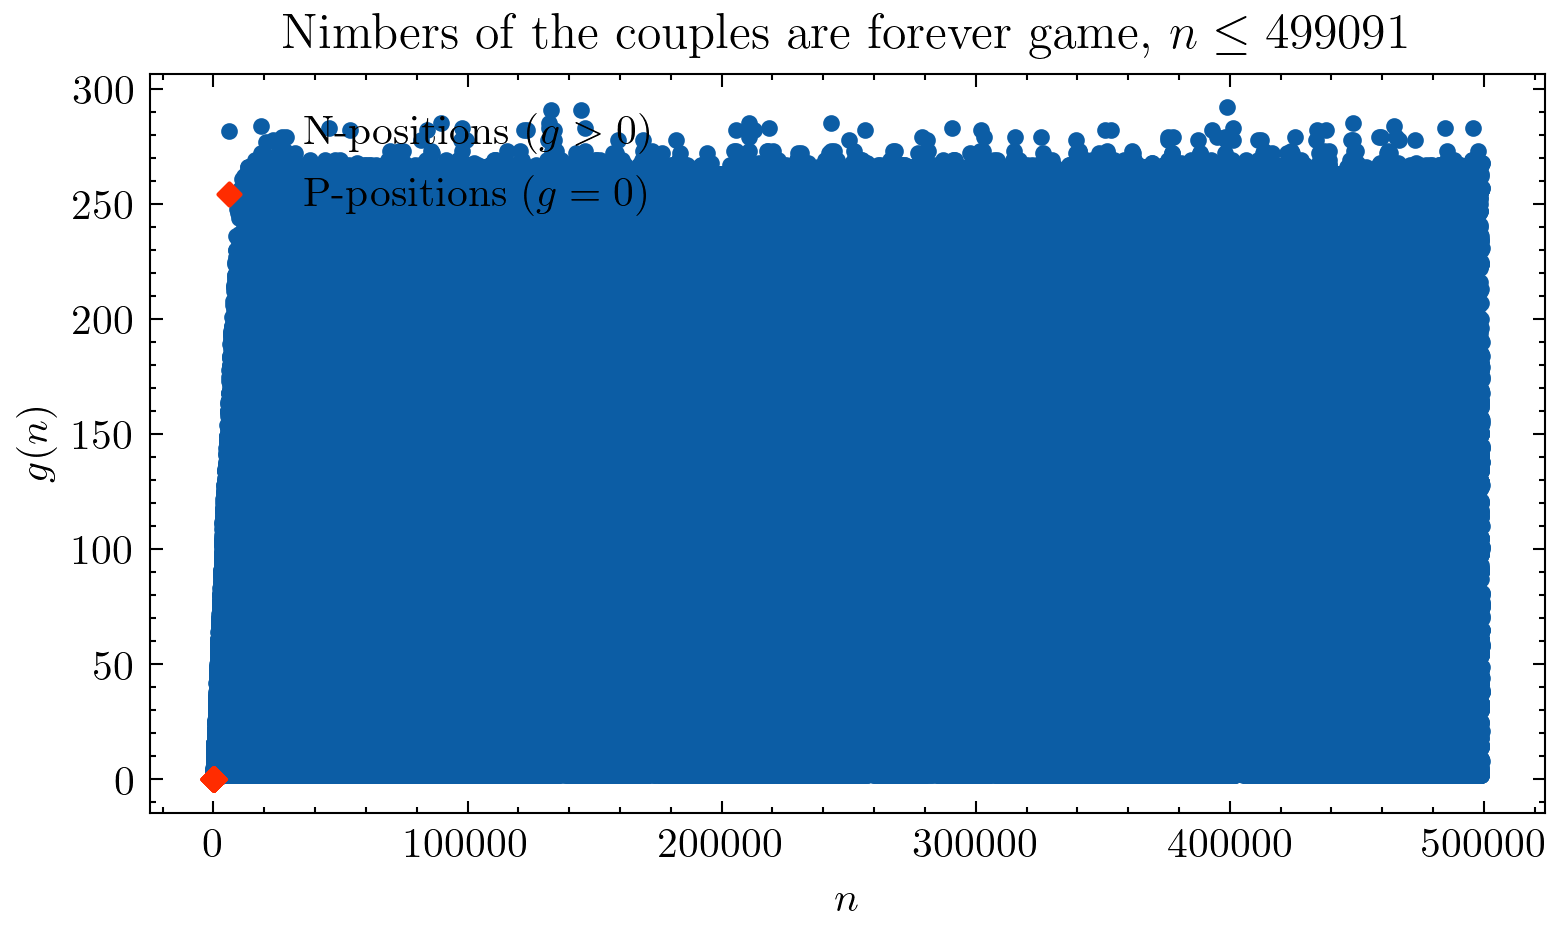
\includegraphics[width=0.75\linewidth]{assets/nimbers.png}};
\end{graphfig}
This graph shows the nimbers for all $N$ up to computational allowment 499091. As the graph shows, there is a plataeu beginning at the sub-100K region and continuing around a value of 275. 
\item Recall the reuls to COUPLES ARE FOREVER! You have a pile of stones. A turn consists of taking a pile and breaking it into smaller piles. You can't touch piles that consist of exactly one stone, or exactly two stones. Find the nimbers for starting piles of 1, 2, 3, 4, 5, and 6 stones.   \color{red}Dang that was a real jump in orders of magnitude from 15 to 500000\color{black} 
\\
\color{blue} RW: The saxophones indeed got louder. At what point do you just go Crypto?\color{black}

\begin{solution}

\begin{table}[H]
    \centering
    \begin{tabular}{c|c}
        1 & 0 \\
        2 & 0 \\
        3 & 1 \\
        4 & 2 \\
        5 & 0 \\
        6 & 1 \\
        7 & 2 \\
        8 & 3 \\
    \end{tabular}
    \caption{Nimbers for the First 8 Starting Stones}\color{red}Yep\color{black}
    \label{tab:placeholder}
\end{table}
\end{solution}

\item An acyclic orientation of a graph is an orientation of the edges such that no cycles are formed. 
\begin{enumerate}[label=\alph*.]
    \item How many acyclic orientations are there of a tree of order n?
    \begin{solution}
        $2^{n-1}$
    \end{solution}
    \begin{proof}
        A tree is always acyclic. Therefore each edge can have it's orientation chosen independently. Therefore, according to the alternate definitions of the tree, a tree has $n-1$ edges, and therefore the number of acyclic orientations are $2^{n-1}$.
    \end{proof}
    \item How many acyclic orientations are there of the paw?
    \begin{solution}
        12
    \end{solution}
    \begin{proof}
        The total case for orientation of the paw is $2^4=16$. However among 16 orientations, we can have a cycle in the three cycle. when we have a cycle we can have 2 cases of cycles (rotating clock wise or the opposite). Additionally, for a single cycle, there are 2 different cases for the edge that goes with the extra leaf. Therefore the number of acyclic orientations are $16-2\times2=12$
    \end{proof}
    \item How many acyclic orientations are there of a 5 cycles?
    \begin{solution}
        30
    \end{solution}
    \begin{proof}
            
        The total case for orientation of 5 cycles is $2^5=32$ . However, among 32 orientations we can have two different kinds of cyclic orientation (rotating clock wise or the opposite). Therefore the number of acyclic orientations are $32-2=30$.\color{red}Good work!\color{black}
    \end{proof}
\end{enumerate}
\item Decompose the Peterson grpah into three isomorphic connected subgraphs. 
\begin{graphfig}{NUM}
    \gpeterson;
\end{graphfig}
\begin{solution}. 
\begin{center}
\begin{graphfig}{}
    \node [v] (a1) at (0, 2){};
    \node [v] (a2) at (2, 1){};
    \node [v] (a3) at (1, -2){};
    \node [v] (a4) at (-1, -2){};
    \node [v] (a5) at (-2, 1){};
    \node [v] (a6) at (0, 1){};
    \node [v] (a7) at (1, 0.5){};
    \node [v] (a8) at (0.5, -1){};
    \node [v] (a9) at (-0.5, -1){};
    \node [v] (a10) at (-1, 0.5){};
    \draw (a5)--(a1)--(a2)--(a3) (a1)--(a6) (a2)--(a7);
\end{graphfig}
\qquad
\begin{graphfig}{}
\node [v] (a1) at (0, 2){};
    \node [v] (a2) at (2, 1){};
    \node [v] (a3) at (1, -2){};
    \node [v] (a4) at (-1, -2){};
    \node [v] (a5) at (-2, 1){};
    \node [v] (a6) at (0, 1){};
    \node [v] (a7) at (1, 0.5){};
    \node [v] (a8) at (0.5, -1){};
    \node [v] (a9) at (-0.5, -1){};
    \node [v] (a10) at (-1, 0.5){};
    \draw (a5)--(a4)--(a3) (a4)--(a9)--(a6) (a9)--(a7);
\end{graphfig}
\qquad
\begin{graphfig}{}
\node [v] (a1) at (0, 2){};
    \node [v] (a2) at (2, 1){};
    \node [v] (a3) at (1, -2){};
    \node [v] (a4) at (-1, -2){};
    \node [v] (a5) at (-2, 1){};
    \node [v] (a6) at (0, 1){};
    \node [v] (a7) at (1, 0.5){};
    \node [v] (a8) at (0.5, -1){};
    \node [v] (a9) at (-0.5, -1){};
    \node [v] (a10) at (-1, 0.5){};
    \draw (a5)--(a10)--(a8)--(a3) (a10)--(a7) (a8)--(a6);
\end{graphfig}
\begin{graphfig}{NUM}\end{graphfig}
\end{center}
\end{solution}\color{red}Good!\color{black}
\\
\color{blue} RW: I really admire the effort that you put into graphing this three times and keeping track of all your vertices. That for sure is the most tedious thing is writing all the edges out in LaTex and just hoping you kept it all straight lol.\color{black}
\item \color{red} \textit{CHALLENGE. }\color{black} How many acyclic orientations are there for $K_5$? How about $K_n$?
\item \color{blue} \textit{UNSOLVED. }\color{black} From Robert Hochberg : The \textit{crossing number} of a graph is the minimum number of edge crossings a representation of the graph has. A planar graph is a graph with a crossing number of zero. $K_{3, 3}$ has a crossing number of one, because you can draw it with only one edge-crossing. Nobody knows the crossing number of $K_{9,9}$. Hochberg found a way to draw it with 256 crossings...can that be beaten? 
\item \color{blue} \textit{UNSOLVED. } \color{black} The Burning Number Conjecture for arbitrary connected graphs. 
\end{enumerate}

\color{blue}( \href{https://www.youtube.com/watch?v=dQw4w9WgXcQ}{Zander please read these additional comments })\color{black}

\color{blue} RW: Really good work on this homework assignment you all! \color{black}
\end{document}